%!TEX TS-program = xelatex
\documentclass[]{friggeri-cv}
\usepackage{fontawesome}
\addbibresource{bibliography.bib}

\begin{document}
\newfontfamily{\FA}[Path = fonts/]{fontawesome-webfont}
\header{Pieter}{ van der Heijden}
       {Software Developer | Software Architect}

% In the aside, each new line forces a line break
\begin{aside}
  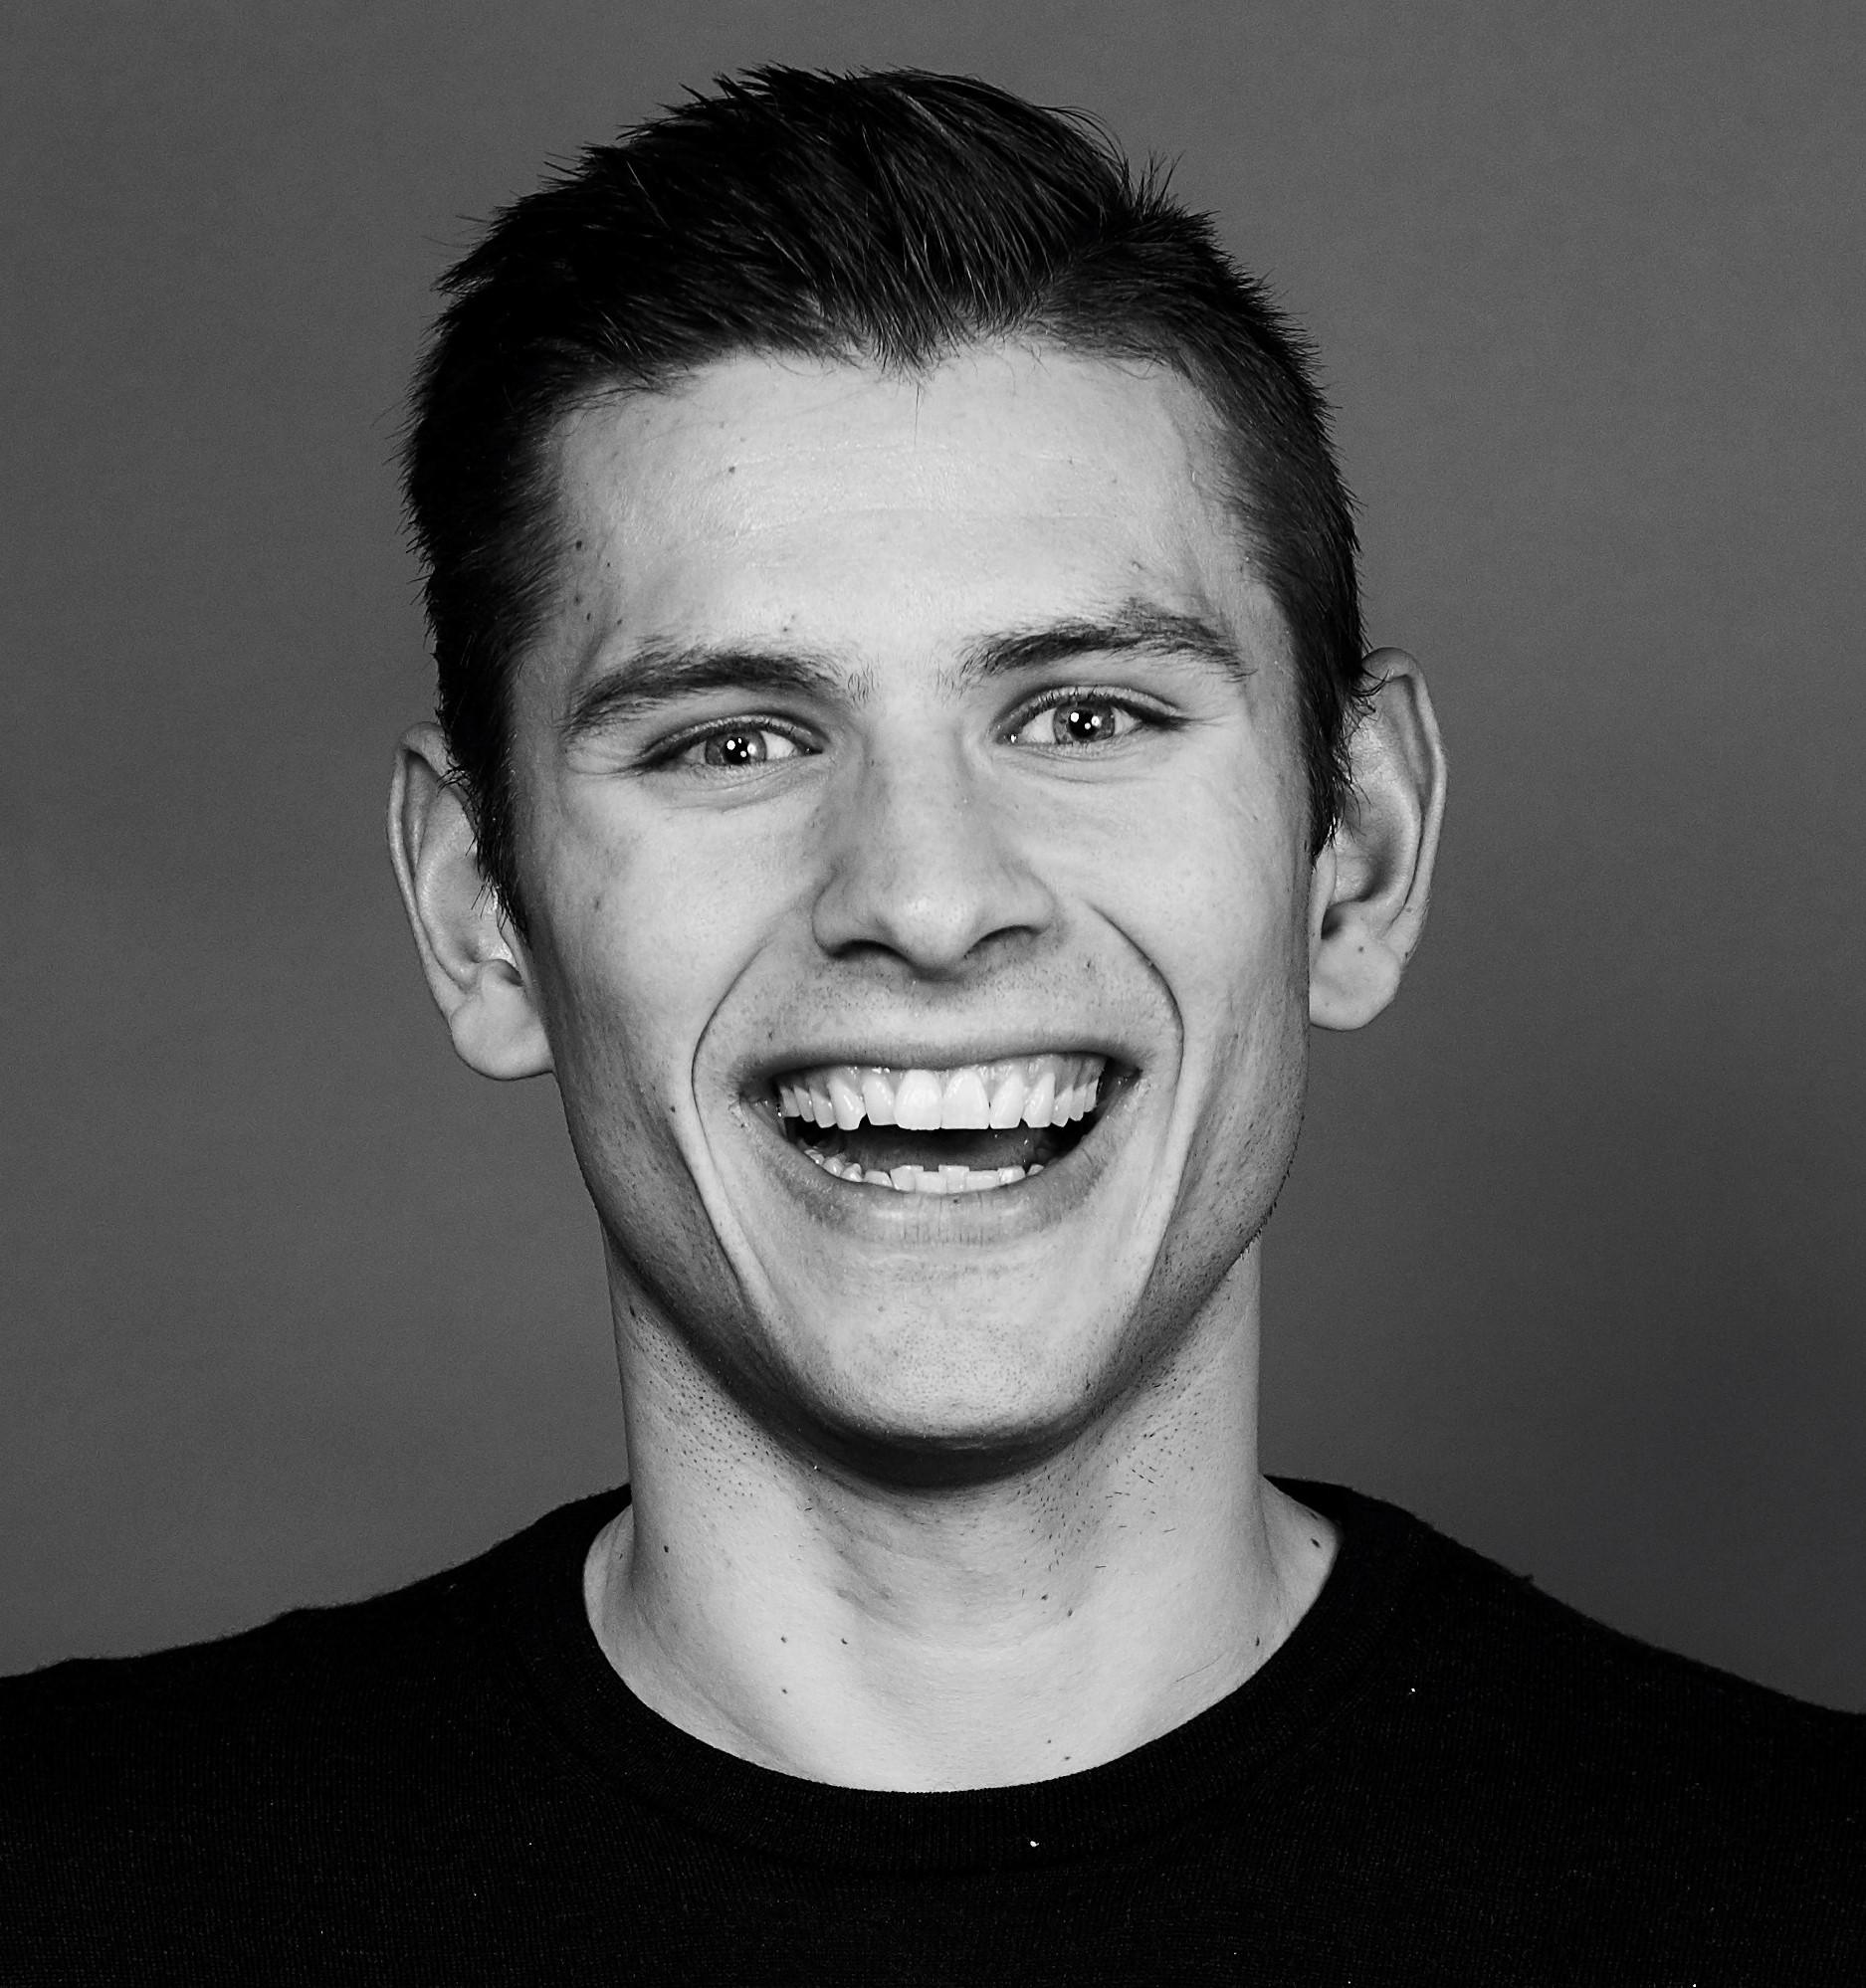
\includegraphics[width=\textwidth]{profilePicture.jpg}
  \section{contact}
    \href{https://www.google.com/maps/place/Tilburg/@51.5737217,4.9686496,12z}{{\FA \faMapMarker}}
    \href{mailto:pietervdheijden@gmail.com}{{\FA \faEnvelope}}
    \href{https://nl.linkedin.com/in/pietervdheijden}{{\FA \faLinkedin}}
    \href{https://github.com/pietervdheijden}{{\FA \faGithub}}
  \section{languages}
    Dutch (native)
    English (professional)
  \section{programming}
    {SQL Server, .NET}
    {CI/CD, DEVOPS}
    {PowerShell}
    {Azure}
    {Docker, Kubernetes}
    {Angular, React}
  \section{hobby}
    Soccer
\end{aside}

\section{about}
Teamplayer, hard-worker, passionate, enthusiastic, enterpreneurial

\section{interests}
SaaS, cloud, management, offshoring.

\section{experience}

\begin{entrylist}
  \entry
    {06-2018 -\\Current}
    {Software Architect}
    {CALVI}
    {Architecture of the complete software suite for all distributed development teams (NL, India and Romania).}
  \entry
    {09-2017 -\\05-2018}
    {Developer}
    {CALVI}
    {Development of high-performing backend systems (DB, API, ETL).}
  \entry
    {09-2016 -\\08-2017}
    {Junior Developer}
    {CALVI}
    {Development of high-performing backend systems (DB, API, ETL).}
  \entry
    {02-2015 -\\03-2016}
    {Software Developer}
    {Freelance (VCF Software Solutions)}
    {Development of the RAET Netto app suite (100k+ downloads)}
  \entry
    {02-2014 -\\11-2014}
    {Mobile and Frontend Developer Trainee}
    {Isaac Software Solutions B.V.}
    {Development of mobile and frontend applications}
\end{entrylist}

\section{certifications \& training classes}
\begin{entrylist}
  \entry
    {2018}
    {Partitioning training class}
    {SQL Skills}
    {IEVLT: Immersion Event on Very Large Tables: Optimizing Performance and Availability through Partitioning}
  \entry
    {2017}
    {Performance tuning training class}
    {SQL Skills}
    {IEPTO1: Immersion Event on Performance Tuning and Optimization – Part 1}
  \entry
    {2016}
    {Microsoft Certified Professional}
    {Microsoft}
    {MS-70461:  Querying Microsoft SQL Server 2012/2014}
\end{entrylist}

\section{education}
\begin{entrylist}
  \entry
    {2013-2016}
    {B.Sc. Software Science}
    {Eindhoven University of Technology}
    {Cum Laude}
  \entry
    {2007-2013}
    {VWO Nature and Technology}
    {Mill-Hill College}
    {Cum Laude}
\end{entrylist}

\end{document}
